\documentclass[11pt,a4paper]{article}
\usepackage[utf8]{inputenc}
\usepackage[T1]{fontenc}
\usepackage[english]{babel}
\usepackage[margin=2.5cm]{geometry}
\usepackage{amsmath,amssymb}
\usepackage{booktabs}
\usepackage{enumitem}
\usepackage{tikz}
\usetikzlibrary{positioning}
\usepackage{hyperref}
\usepackage{xcolor}
\hypersetup{colorlinks=true, linkcolor=black, urlcolor=blue!60!black}
\setlist{nosep}
\newcommand{\code}[1]{\texttt{#1}}

\title{SCuLPT Vision: project scope so far}
\author{Carla González Mina}
\date{\today}

\begin{document}
\maketitle

\section{What I am trying to do}

SCuLPT is a tangible programming language. A program is a sculpture built from 3D-printed blocks, and SCuLPTER is the text interpreter that runs it. Until now, going from the sculpture to the text has been the user's job. What I want is to remove that step, so that one or two cameras pointed at the physical blocks are enough to reconstruct the program they form and run it on the real interpreter, without changing the language itself.

One rule I set from the start and have kept is that the files that define the language (\code{Tokens}, \code{Lexer}, \code{Parser}, \code{AST}, \code{Interpreter}) are never touched. The prototype uses them exactly as they are, both from Python through \code{scala-cli} and compiled to JavaScript with Scala.js for the simulator.

Everything lives in \code{vision-prototype/}. Figure~\ref{fig:pipeline} shows the whole path, and the rest of this document walks through each stage in the order the image travels through them.

\begin{figure}[h]
\centering
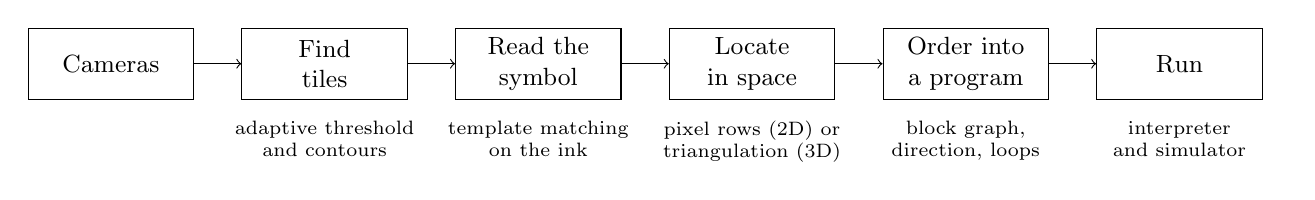
\begin{tikzpicture}[node distance=6mm, every node/.style={font=\small}]
  \node[draw, minimum height=9mm, minimum width=21mm, align=center] (cam) {Cameras};
  \node[draw, minimum height=9mm, minimum width=21mm, align=center, right=of cam] (reg) {Find\\tiles};
  \node[draw, minimum height=9mm, minimum width=21mm, align=center, right=of reg] (rec) {Read the\\symbol};
  \node[draw, minimum height=9mm, minimum width=21mm, align=center, right=of rec] (pos) {Locate\\in space};
  \node[draw, minimum height=9mm, minimum width=21mm, align=center, right=of pos] (prog) {Order into\\a program};
  \node[draw, minimum height=9mm, minimum width=21mm, align=center, right=of prog] (run) {Run};
  \draw[->] (cam) -- (reg);
  \draw[->] (reg) -- (rec);
  \draw[->] (rec) -- (pos);
  \draw[->] (pos) -- (prog);
  \draw[->] (prog) -- (run);
  \node[below=1.5mm of reg, align=center, text width=25mm, font=\scriptsize] {adaptive threshold\\and contours};
  \node[below=1.5mm of rec, align=center, text width=25mm, font=\scriptsize] {template matching\\on the ink};
  \node[below=1.5mm of pos, align=center, text width=25mm, font=\scriptsize] {pixel rows (2D) or\\triangulation (3D)};
  \node[below=1.5mm of prog, align=center, text width=25mm, font=\scriptsize] {block graph,\\direction, loops};
  \node[below=1.5mm of run, align=center, text width=25mm, font=\scriptsize] {interpreter\\and simulator};
\end{tikzpicture}
\caption{The pipeline. Every reading, live or from a saved image, goes through the same five stages.}
\label{fig:pipeline}
\end{figure}

\section{What a block looks like to the camera}

Each block carries an \emph{operation tile} on its raised end and one or two \emph{parameter tiles} after it (Figure~\ref{fig:block}). On the blocks the symbols are hand-drawn with a marker. An arrow pointing down means \code{PUSH}, a plus sign means \code{ADD}, a heart or a circle names a stack, and digits are literals. A small table, \code{simbolos.json}, maps each hand-drawn symbol to the lexeme the interpreter expects and says whether it is an operation, a stack or a literal. Stack names have to be plain ASCII identifiers because the lexer accepts nothing else, so the heart is emitted as \code{heart} and the circle as \code{circle}.

The order of the tiles on the block is not decoration. The operation comes first and the parameters follow it, and that is also the direction in which the program flows into the next block. This single fact is what later lets me recover the reading direction of a whole chain.

\begin{figure}[h]
\centering
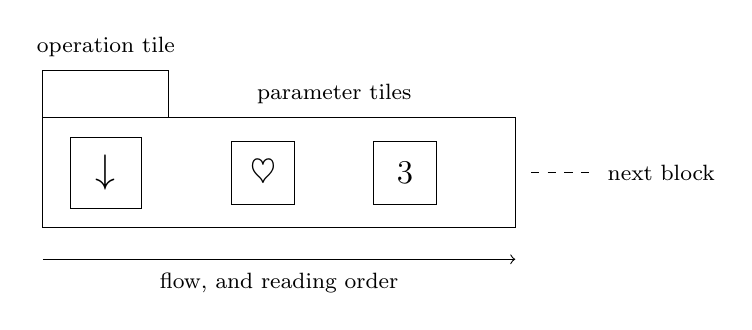
\begin{tikzpicture}[x=1mm, y=1mm, every node/.style={font=\small}]
  \draw (0,0) rectangle (60,14);
  \draw (0,14) rectangle (16,20);
  \node[draw, minimum size=9mm, font=\Large] at (8,7) {$\downarrow$};
  \node[draw, minimum size=8mm, font=\large] at (28,7) {$\heartsuit$};
  \node[draw, minimum size=8mm, font=\large] at (46,7) {3};
  \node[above, font=\footnotesize] at (8,20.5) {operation tile};
  \node[above, font=\footnotesize] at (37,14.5) {parameter tiles};
  \draw[->] (0,-4) -- (60,-4);
  \node[below, font=\footnotesize] at (30,-4.5) {flow, and reading order};
  \draw[dashed] (62,7) -- (70,7);
  \node[right, font=\footnotesize] at (70.5,7) {next block};
\end{tikzpicture}
\caption{One block as the pipeline sees it. This one reads \code{PUSH heart 3}.}
\label{fig:block}
\end{figure}

\section{Finding the tiles}

I do not look for the blocks themselves, only for the tiles, because the tile is where the information is. The frame is converted to greyscale, blurred slightly, and turned into black and white with an \emph{adaptive threshold}. Instead of comparing every pixel against one global value, each pixel is compared against the average of its own neighbourhood (a $35\times35$ window). A dark stroke on a light tile stands out under a lamp and in shadow alike, which is what makes this tolerate the uneven lighting of a real table. The outlines of the resulting black shapes are the candidate regions.

Most of those candidates are not tiles, so three simple checks throw out anything that cannot be one. A region is dropped if it covers less than $0.2\%$ or more than $15\%$ of the frame, or if it is much wider than tall (aspect ratio above $1.8$). That gets rid of the cardboard box, the edge of the table and the speckle noise before any comparison is attempted.

\section{Reading the symbol}

Each remaining region is compared against a reference photo of every symbol, and the best match wins. The comparison is a normalised correlation. In words, it measures how well the light and dark pattern of the region lines up with the pattern of the template, after removing the overall brightness of each. For a region $I$ and a template $T$ of the same size it is
\[
  \rho(I,T) = \frac{\sum (I-\bar I)(T-\bar T)}{\sqrt{\sum (I-\bar I)^2 \,\sum (T-\bar T)^2}},
\]
a number between $-1$ and $1$, where $1$ means identical up to brightness and contrast. It does not tolerate rotation, and it does not know which part of the picture matters. Both problems needed a fix.

\paragraph{Compare ink, not tiles.} My first version compared whole tiles, and the templates for \code{ADD} and \code{SUB} correlated at $0.87$ with each other. The outline of the square tile dominated the sum and the stroke barely counted, so almost any square blob passed as some symbol. Now both the region and every template are reduced to their ink before comparing. I ignore a thin border (the edge of the tile and its shadow), separate the dark marker from the light tile with Otsu's method (it picks the threshold automatically from the image's own histogram, so there is no hand-tuned value), crop to the box that contains the stroke, pad it to a square so the shape is not distorted, and resize it to $64\times64$. After this, \code{ADD} versus \code{SUB} drops to $0.65$, and a region with no ink at all is discarded without comparing anything.

\paragraph{Rotation bank.} Plain correlation breaks past roughly $20^\circ$ of rotation, so every template is stored rotated from $-40^\circ$ to $+40^\circ$ in $8^\circ$ steps, and a symbol's score is the best over its bank.

\paragraph{Accept only clear winners.} A region is read as symbol $s$ only if its score is at least $0.45$ and it beats the runner-up by at least $0.08$. The margin is what kills false positives. A blob that looks $0.47$ like \code{JMP} and $0.45$ like \code{MOV} looks like neither, and it is better to read nothing than to read the wrong thing. Both constants were set by hand and will be tuned with the dataset of Section~\ref{sec:eval}.

\section{Locating the tiles}

There are two ways to do this, and I have both.

\subsection{Flat programs, no calibration}

With one or more uncalibrated cameras, \code{reconstruir.py} sorts the detections by their vertical pixel position, groups the ones that sit on the same line (within $40$\,px) into a row, and orders each row from left to right. A row is one instruction. When several cameras are connected, each one is read on its own and the view that recognises the most symbols wins. A reading is only reported once nothing has moved for almost a second, so a half-built program is never executed. It is simple and works for programs lying flat, but it knows nothing about depth or about blocks stacked on top of each other.

\subsection{Sculptures, two calibrated cameras}

Two cameras that know their own optics and where they are relative to each other can turn a pair of pixel positions into a point in millimetres. That is what \code{triangulate.py} does.

\paragraph{Calibration.} Each camera is first calibrated on its own by showing it a chessboard (nine by six inner corners, $25$\,mm squares) from at least fifteen angles. This yields its intrinsic matrix $K$ (focal length and image centre) and its lens distortion. Then both cameras see the board at once, which yields the rotation $R$ and translation $t$ from camera A to camera B. This has to be redone if either camera moves.

\paragraph{Matching a tile between the two views.} For a tile seen in camera A, its image in camera B cannot be anywhere. It must lie on one specific line, the \emph{epipolar line}, which I get from the fundamental matrix
\[
  F = K_b^{-\top}\,[t]_\times\, R\, K_a^{-1}, \qquad \ell_b = F\,x_a .
\]
A candidate in B is accepted only if it lies within $15$\,px of that line. This alone rules out most wrong pairings between repeated symbols, but not all of them. Several \code{PUSH} tiles in one row, seen by two cameras placed side by side, all fall on the same line. What tells them apart is depth. A wrong pairing triangulates to a point hundreds of millimetres above or below the table, so I add to the cost of each pairing how far its depth is from the depth of the symbols that were not ambiguous, and pick the assignment with the lowest total cost.

\paragraph{Triangulation and the table frame.} Each matched pair is triangulated into a 3D point in the frame of camera A. Since camera A is tilted, I then move everything into a \emph{table frame}, with $x$ and $y$ along the surface and $z$ pointing up. The frame comes for free from the calibration. In the first stereo sample the chessboard lies on the table, and its pose is the table's pose. If a calibration file was made without that, the prototype falls back to fitting a plane through the detected tiles themselves, which is exact for a flat program and only approximate for a tall sculpture.

\section{Ordering tiles into a program}

This is the part that encodes what a SCuLPT program physically is. \code{adjacency.py} receives labelled 3D points and answers three questions. Which tiles belong to the same block, in what order the blocks are read, and whether the chain closes on itself.

\paragraph{Which blocks are connected.} Operation tiles are separated from parameter tiles using the symbol table. Two operation tiles are neighbours when their distance is one block pitch, $60 \pm 15$\,mm (the pitch of the STL models; I still have to measure it on the printed blocks, including through a T connector). This gives a graph whose nodes are blocks and whose edges are physical connections.

\paragraph{Which way to read it.} Nothing in the graph says which loose end is the start, and at a T junction nothing says which branch continues. So I simply try every possibility. Every walk through the graph is generated, branching at each choice, and linear walks are also tried backwards. Then the parameter tiles decide. Under the correct orientation every parameter tile sits just \emph{ahead} of its operation along the flow (Figure~\ref{fig:block}), so for each candidate walk I attach every tile to the block it falls behind, and the walk under which the tiles fit best wins. My first version attached each tile to the nearest operation instead, and it failed in an obvious way once I looked at it. With a $60$\,mm pitch, a tile in the middle of a block is as close to the next operation as to its own. Turning the direction into the hypothesis that best explains where the tiles are is what fixed it. When a chain has no parameter tiles at all, forwards and backwards look the same and the program is emitted with a \emph{direction unconfirmed} warning.

\paragraph{Loops become jumps.} A cycle of blocks closed with a T connector is a structural loop, and the text language has no syntax for it. It is written with a backward jump instead. If a walk ends next to a block it already visited, that block is the loop entry, and I append a \code{JMP} whose offset is the entry's position minus the jump's own position. The offset follows how the interpreter moves its program counter, and I checked it by running a reconstructed loop and watching the counter land back on the entry block.

\paragraph{What comes out.} Besides the text of the program, each instruction carries the position of its operation tile, the direction of the flow and the positions of its parameters. The jump that stands in for a loop has no block of its own and is marked as virtual. That is what the simulator uses to draw the sculpture where it actually is.

\section{Running and showing it}

The reconstructed text goes to the real Scala interpreter, which prints the state of every stack after each step, or the reason the program is invalid. At the same time, a virtual table built with three.js shows the blocks with their real STL geometry. Every change there is re-validated by the interpreter compiled to JavaScript, so a hand-built program and a camera reading go through the same code. A 2D reading brings only instructions and is laid out in a grid. A 3D reading brings positions, and the scene places each block at its coordinates, rotated to follow the flow, with the virtual \code{JMP} of a loop drawn as a return curve from the last block to the loop entry.

\section{Measuring instead of guessing}
\label{sec:eval}

Thresholds cannot be tuned by looking at one image, so the prototype has its own measurement loop. \code{capture\_dataset.py} saves frames labelled with the program that was on the table, who drew the tiles and when. \code{evaluar\_dataset.py} runs the same detection as the live pipeline over each saved image and compares what was read with what was there. For each symbol it counts how many were found correctly, how many were invented and how many were missed, and turns that into precision, recall and $F_1$, per symbol and overall. It also reports how many programs came out exactly right and, most useful of all, a confusion list saying what was read in place of what. A symbol that is often missed needs a better reference photo or a lower threshold. Two symbols that are confused with each other need to be drawn more differently.

A set of 22 automated tests runs without any camera. They cover the reconstruction from synthetic point sets (chains, reversed chains, loops with and without a prefix, isolated blocks), the whole stereo pipeline with two virtual cameras looking at a known program with repeated symbols in shuffled order (the program must come back exactly and every point within a millimetre), the classifier (every template recognises itself with margin, while noise, blank regions and filled squares are rejected), the region filters, the table frame and the evaluator.

\section{Where it stands}

\begin{center}
\begin{tabular}{@{}lll@{}}
\toprule
Component & Status & Checked against \\
\midrule
Hand-drawn symbol table & done & photo of the blocks \\
Classifier (ink + margin + filters) & done & render templates, tests \\
2D reconstruction + interpreter & done & synthetic image, real cameras \\
Stereo calibration and triangulation & done & virtual cameras (tests) \\
Points $\to$ program (direction, loops) & done & synthetic points, real interpreter \\
Simulator with real positions & done & not visually checked yet \\
Recognition metrics & done & synthetic dataset \\
Templates from the real blocks & \textbf{pending} & --- \\
Real block pitch (straight and through a T) & \textbf{pending} & --- \\
Calibration with the real cameras & \textbf{pending} & --- \\
\bottomrule
\end{tabular}
\end{center}

Everything pending is physical, and the order matters. Without photos of the real tiles no reconstructed program is valid, because the current templates come from the render, do not match the hand-drawn symbols, and produce false positives. After that come the first real reading, a dataset with more than one person drawing the tiles, calibration with the board lying flat on the table, and measuring the block pitch.

The limits I already know about are these. Template matching depends on lighting and on the stroke being clearly darker than the tile. The 2D reconstruction cannot tell heights apart. The 3D one assumes that ambiguous matches can be resolved by depth. And without a recorded board pose the table frame is fitted to the points themselves, which is only approximate for a tall sculpture.

\end{document}
